\chapter{Methodology}
%This chapter should discuss the details of your implementation for the assignment. 
%Everything related to \emph{how} things were done should go here.
%Remember to avoid going into too much details, summarize appropriately and try to use figures/charts.
%Make sure you refer to the figures (such as Figure \ref{fig:universe}) and charts you add in the text.
%Avoid putting lots of source code here -- small code snippets are fine if you want to discuss something specific.
\section{Presentation of the solution}
The choosen algorithm for this project was to use the Montgomery Exponentiation method. For our RSA circuit we chose to implement one module for the MonPro operation, a datapath module with various registers for storing inputs and intermediate results and a top-level controller module with a state machine and control signals for the datapath.\\
In order to use Montgomery's algorithm without taking additional parameters, a simplified version of Blakley's algorithm was used to compute the following required input parameters:
\begin{equation}
    \bar{x}=1*R*mod(n), R=2^{128}
\end{equation}
\begin{equation}
    \bar{M}=M*R*mod(n), R=2^{128}
\end{equation}

The top level implementation is as seen in figure \ref{fig:toplevel}. The datapath takes the input data 32-bits at a time and these signals are then loaded into the correct registers, based on control signals from the top level ControlFSM.\\
To make data loading easier, a modified version of the register supplied in the module library was created with an additional load\_enable pin. This allowed for the use of a common input data bus, instead of shift registers or a tree of demultiplexers to route the data. The code for this register can be seen in appendix \ref{app:register_enable_reset_n}.\\
The state machine keeps track of the inputs and states of various registers, and is responsible for starting the different operations at the right time, while setting control signals for routing the results into the correct registers.\\
It's implemented as a Mealy machine\cite{mealy}, and sends control signals to the datapath which actually routes and stores the data. A simplified state diagram (without output signals) can be seen in figure \ref{fig:statediagramrsa}.


\begin{figure}[H]
\centering
\includegraphics[width=\textwidth]{images/TopLevel}
\caption{A top-level overview of the RSA circuit.}
\label{fig:toplevel}
\end{figure}


\subsection{Blakley module}
In our case, the Blakley module is only needed for data preprocessing before the main algorithm can start working. Because of this a simplified Blakley module was implemented, based on assumptions about the input.\\
The module is implemented with combinational arithmetics, and an internal iteration counter is used to determine when the computations are complete and the 'complete' signal can be sent. The result data gets propagated to the output bus immediately after each cycle.\\
In hindsight the combinational and sequential parts should probably have been split into separate processes, but it worked satisfactory to fullfill its purpose in this case.\\
However, when uploaded to the FPGA for testing it would not synthesize.

\subsection{Monpro module}
Much like the Blakley module it is implemented using combinational arithmetics, but in addition there is a more clear separation between the synchronous and combinational parts as some combinational feedback previously occurred when running multiple iterations in a row.\\
Here, the result and 'complete' signal output was also delayed by one clock cycle in an attempt to reduce the potential for combinational feedback problems.

\subsection{Stitching everything together}
The different modules were combined by creating instances and connecting them with signals and port maps. Muxes and processes for routing and propagating control signals were also required.
As the code grew testing and verification of the combined "super-modules" quickly became increasingly challenging, so keeping things as separated as practically possible was important.\\ 
The ControlFSM module mainly consists of two processes (in addition to smaller ones for f.i. simple muxes); one combinational process for deciding what the next state should be and which control signals should be sent next, and one synchronous process responsible for updating the outputs on the next clock.
\\
The RSA module ended up having the states listed in table \ref{tab:states}.\\

\begin{table}[H]
    \centering
    \begin{tabular}{|l|l|}
    \hline
        IDLE & The system waits for the next command from the outside \\ \hline
        LOAD\_CONFIG & The system loads the config parameters from the DataIn bus, before using\\ & the Blakley module to generate the starting point for the ciphertext\\ \hline
        LOAD\_MESSAGE & The system loads the message from the DataIn bus, before using the\\ & Blakley module to transform the message into the Montgomery domain \\ \hline
        WAIT\_MONPRO & The system waits for the Monpro module to complete one iteration \\\hline
        RUN\_MONPRO   & The system starts the next iteration of Monpro. \\\hline
        OUTPUT\_DATA & The system is done encrypting/decrypting the message and\\ & returns the result to the DataOut bus \\ \hline
    \end{tabular}
    \caption{States of RSA module}
    \label{tab:states}
\end{table}

\begin{figure}[H]
\centering
\includegraphics[width=\textwidth]{images/StateDiagram}
\caption{State diagram for RSA module}
\label{fig:statediagramrsa}
\end{figure}
%%
%Add content in this section that describes how you tested and verified the correctness of your implementation, with respect to the requirements of the assignment.

\section{Verification plan}
%- Write a verification plan.\\
%- What metrics will you use to decide when you are done verifying?
%(pass rate, code coverage, functional coverage).\\
%- Demonstrate the use of assertions \\
%- What bring up test strategy have you planned?\\ 
%- Discuss/Analyze/Conclude\\
Before starting to implement the actual VHDL code, the algorithm had to be verified. For this, a simple python program was written that implemented the desired behavior:

\inputminted[firstline=45,lastline=56]{python}{../Project/monexp.py}

This was then used alongside the simulator and waveform window to check that the output actually matched what it was supposed to be at any given time, and was a great aid in debugging, see figure \ref{fig:waveform}.\\
\begin{figure}[H]
\centering
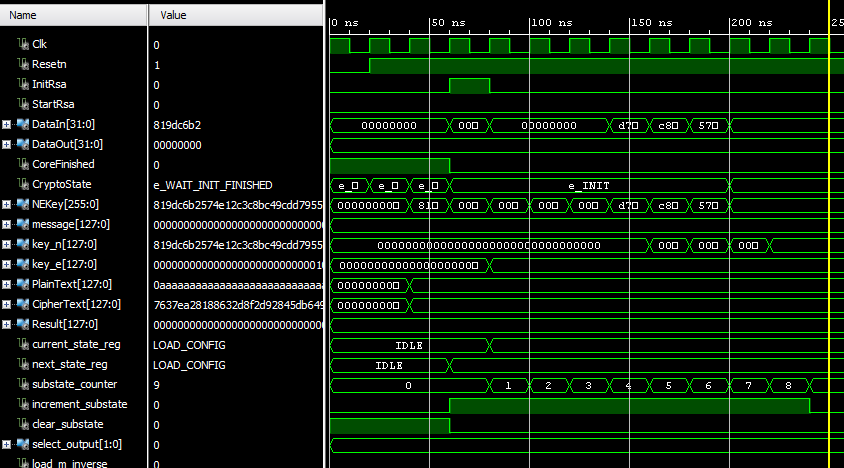
\includegraphics[width=\textwidth]{images/Vivado_waveform}
\caption{Waveform simulation from Vivado}
\label{fig:waveform}
\end{figure}
Each submodule of the design was verified with its own testbench. % TODO: add source ref.
The RSAcore module was verified using the testbenches provided for the course.
\\
Improvements in the verification plan would have been to use Bitvis library, but this would have required a different VHDL compiler than Vivado. \\
Assertions in the testbench code would also have been a possible (and somewhat simpler) solution; even if it doesn't provide the same level of progress information and positive acknowledgement, it at least lets you know when something happened.